\chapter{Diseño e implementación} % Main chapter title
En este capitulo se abordara la descripcion de la arquitectura general del sistema, arquitectura del firmware, detalles de los controladores desarrollados para el modulo de comunicaicon y los sensores, desarrollo del hardware y la configuracion de la plataforma IoT. 
\label{Chapter3} % Change X to a consecutive number; for referencing this chapter elsewhere, use \ref{ChapterX}

\definecolor{mygreen}{rgb}{0,0.6,0}
\definecolor{mygray}{rgb}{0.5,0.5,0.5}
\definecolor{mymauve}{rgb}{0.58,0,0.82}

%%%%%%%%%%%%%%%%%%%%%%%%%%%%%%%%%%%%%%%%%%%%%%%%%%%%%%%%%%%%%%%%%%%%%%%%%%%%%
% parámetros para configurar el formato del código en los entornos lstlisting
%%%%%%%%%%%%%%%%%%%%%%%%%%%%%%%%%%%%%%%%%%%%%%%%%%%%%%%%%%%%%%%%%%%%%%%%%%%%%
\lstset{ %
  backgroundcolor=\color{white},   % choose the background color; you must add \usepackage{color} or \usepackage{xcolor}
  basicstyle=\footnotesize,        % the size of the fonts that are used for the code
  breakatwhitespace=false,         % sets if automatic breaks should only happen at whitespace
  breaklines=true,                 % sets automatic line breaking
  captionpos=b,                    % sets the caption-position to bottom
  commentstyle=\color{mygreen},    % comment style
  deletekeywords={...},            % if you want to delete keywords from the given language
  %escapeinside={\%*}{*)},          % if you want to add LaTeX within your code
  %extendedchars=true,              % lets you use non-ASCII characters; for 8-bits encodings only, does not work with UTF-8
  %frame=single,	                % adds a frame around the code
  keepspaces=true,                 % keeps spaces in text, useful for keeping indentation of code (possibly needs columns=flexible)
  keywordstyle=\color{blue},       % keyword style
  language=[ANSI]C,                % the language of the code
  %otherkeywords={*,...},           % if you want to add more keywords to the set
  numbers=left,                    % where to put the line-numbers; possible values are (none, left, right)
  numbersep=5pt,                   % how far the line-numbers are from the code
  numberstyle=\tiny\color{mygray}, % the style that is used for the line-numbers
  rulecolor=\color{black},         % if not set, the frame-color may be changed on line-breaks within not-black text (e.g. comments (green here))
  showspaces=false,                % show spaces everywhere adding particular underscores; it overrides 'showstringspaces'
  showstringspaces=false,          % underline spaces within strings only
  showtabs=false,                  % show tabs within strings adding particular underscores
  stepnumber=1,                    % the step between two line-numbers. If it's 1, each line will be numbered
  stringstyle=\color{mymauve},     % string literal style
  tabsize=2,	                   % sets default tabsize to 2 spaces
  title=\lstname,                  % show the filename of files included with \lstinputlisting; also try caption instead of title
  morecomment=[s]{/*}{*/}
}


%----------------------------------------------------------------------------------------
%	SECTION 1
%----------------------------------------------------------------------------------------
\section{Diagrama de bloques general del sistema}

En la figura \ref{fig:Diagrama general del sistema IoT} se muestra el diagrama en bloques general del sistema implementado donde se describe la arquitectura IoT la cual consta de tres capas: percepción, red y aplicación.

\begin{figure}[htbp]
	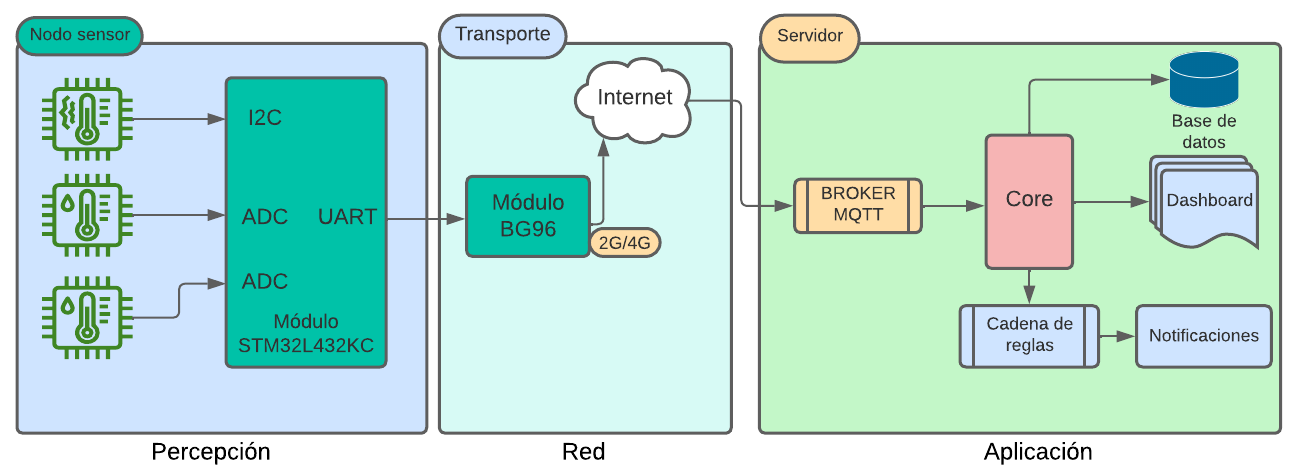
\includegraphics[width=1\textwidth]{./Figures/DiagramaDelSistema.png}
	\caption{Diagrama general del sistema IoT.}
	\label{fig:Diagrama general del sistema IoT}
\end{figure}

En cada una de las capas, se despliegan tecnologias y componentes de hardware y software. A continuación se describe cada una de ellas.

\begin{itemize}
	\item Capa de percepción. En la capa de percepción, los nodos sensores son los encargados de medir variables ambientales, hacer un prepocesamiento y enviarlas a la capa de red. Para su desarrollo se utilizo la placa STM32L432KC que contiene el firmware del sistema,tambien consta de un sensor de humedad y temperatrua ambiente AHT10 que se comunica con la placa de desarrollo mediante el protocolo I2C, sensor de humedad de suelo HL-69 y el sensor de luz UV ML-18 que se comunicacion con el modulo mediante entradas analogicas.
  \item Capa de red. En cuanto a la red, se utilizo un modulo quectel BG96 que puede conectarse a la red 2G, 4G, NB-IoT automaticamente dependiendo del nivel de la red en el lugar de la implementacion del modulo sensor, se comunica con el microcontrolador por comandos AT por puerto UART.
  \item Capa de aplicación. En la capa de aplicacion, se utilizo ThingsBoard como plataforma IoT que nos brinda los microservicios de broker MQTT como puerta de entrada al servidor, base de datos para el almacenamiento, nos brinda la interfaz grafica para la visualizacion de los datos y nos permite gestionar la alarmas del sistema.


\end{itemize}

\section{Arquitectura de firmware}
El desarrollo del firmware fue la tarea mas compleja del proyecto debido a que uno de los objetivos fue lograr 
El firmware fue estructurado en capas como se muestra en la figura \ref{fig:Capas del firmware} se dividio el firmware en capas para facilitar el desarrollo y reducir la complejidad del codigo escritolo separo en capas 

\begin{figure}[htbp]
  \centering
	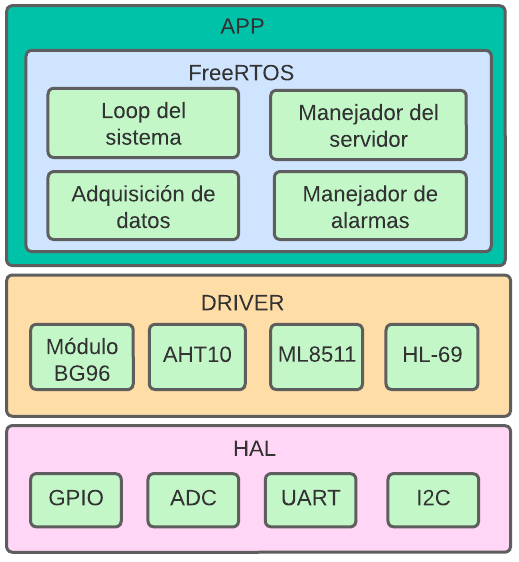
\includegraphics[width=0.7\textwidth]{./Figures/Capas del firmware.png}
	\caption{Capas del firmware.}
	\label{fig:Capas del firmware}
\end{figure}

 La capa Base es la mas baja del sistema y esta compuesta por la libreria HAL de STM, proporciona a las capas superiores la capacidad de interactuar con los perifericos del  microcontrolador STM32L432KC atraves de funciones en lenguaje C
  \begin{itemize}
    \item GPIO: La API proporciona funciones para definir el estado de los pines del microcontrolador.Fueron utilizadas por la capa de APP para el control de los leds de debug del sistema y para el encendido y reset del modulo de comunicacion. Las funciones de esta libreria fue utilizada por la capa de APP para gestionar las entradas y salidas del microcontrolador.
    \item ADC: Proporcionan funciones para la configuracion, lectura y escritura de los pines de microcontroladora senales analogicas. Se utilizaron estas funciones para hacer la lectura de los sensores de humedad de suelo y el sensor de luz UV.
    \item UART: Brinda funciones para la lectura y estritura por el puerto UART del microcontrolador.El firmware utiliza estas funciones para la comunicacion con el modulo BG96.
    \item I2C:Proporciona funciones para la lectura y escritura por protocolo I2C.El driver del sensor de AHT10 utiliza estas funciones para hacer la lectura de los datos.Se utilizaron estas funciones para la lectura de los datos del sensor de AHT10.
    
  \end{itemize}


La capa DRIVERS esta compuesta por los modulos que se desarrollaron para hardware externo al microcontrolador que permiten al microcontrolador enteractuar con hardware externo.Se desarrollaron drivers para el modulo de comunicacion BG96,AHT10,ML18 y HL69
\begin{itemize}
  \item Modulo BG96:Se desarrollo el driver para el modulo BG96, para establecer la comunicacion de este elemento con el microcontrolador a traves del puerto UART.Las funciones mas importantes que proporcionan son
  \begin{itemize}
    \item Estado del modulo.
    \item Descripcion del modulo.
    \item Configuracion APN de la red.
    \item Conexion TCP.
    \item Conexion a broker MQTT.
  \end{itemize}
  \item AHT10: Se desarrollo utilizando la hoja de datos del sensor, proporciona las funciones mas importante inicializacion y lectura de los valores obtenidos por el sensor.
  \item ML18: Se escribio una funcion que permite convertir los datos obtenidos de forma analogica a valores significativos de humedad.
  
\end{itemize}

La capa de APP es la de mayor nivel gerarquico.Se la desarrollo sobre freeRTOS que nos permite hacer un codigo mas escalable.
Se implementaron cuatro tareas
\begin{itemize}
    \item Loop del sistema: Esta tarea es la que nos da la secuencialidad del sistema.
    \item Conexion servidor: Se encarga de manejar la conexion a la red y al broker MQTT.
    \item Adquisicion de datos: Se encarga de hacer la lectura de los sensores.
    \item Manejador de eventos: Esta tarea se encarga de manejar todos lo eventos del sistema.
  \end{itemize}

\section{Desarrollo del firmware}
Para el desarrollo del firmware se utilizo el IDE oficial de STMicroelectronic(STM32CubeIDE).

El firmware fue desarrollado sobre freeRTOS, se utilizaron algunas de sus funcionanlidades como queue, semaforos, tareas, interrupciones.




En la figura se describe las diferentes tareas que se crearon para el firmware y la comunicacion entre las mismas.


El firmware tiene una etapa de inicializacion en la figura podemos ver la secuancia de inicializacion del sistema.

Luego el firmware da el control del sistema al sistema operativo y permanece ejecutando de forma continua las tareas creadas en la etapa de inicializacion del sistema 


En la figura \ref{fig:Df inicio firmware}  se muestra en diagrama de flujo de inicion del firmware.

\begin{figure}[htbp]
  \centering
	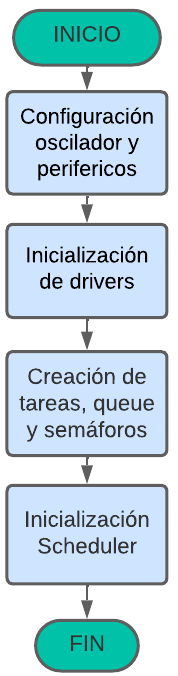
\includegraphics[width=0.25\textwidth]{./Figures/DF inicio firmware.png}
	\caption{Diagrama de flujo inicio firmware.}
	\label{fig:Df inicio firmware}
\end{figure}

Descripcion de los bloques del diagrama.

Lo primero que el firmware realiza es la configuracion del hardware del microcontrolador, luego se inicializan los drivers del modulo de comunicacion celular BG96 y el driver del sensor de humedad AHT10, ejecutan las funciones de inicializacion de los sensores y del modulo de comunicacion celular,posteriormente se crean las tareas, queues y los semaforos del sistema y finalmente se da el contro del sistema al scheduler del sistema operativo. 

Para el control del sistema se crearon cuatro tareas sobre freeRTOS, que se comunican y sincronizan atraves de colas y semaforos en la figura la comunicacion entre tareas.

A continuacion se desarrollara a implementacion de cada tarea del sistema.

\begin{figure}[htbp]
  \centering
	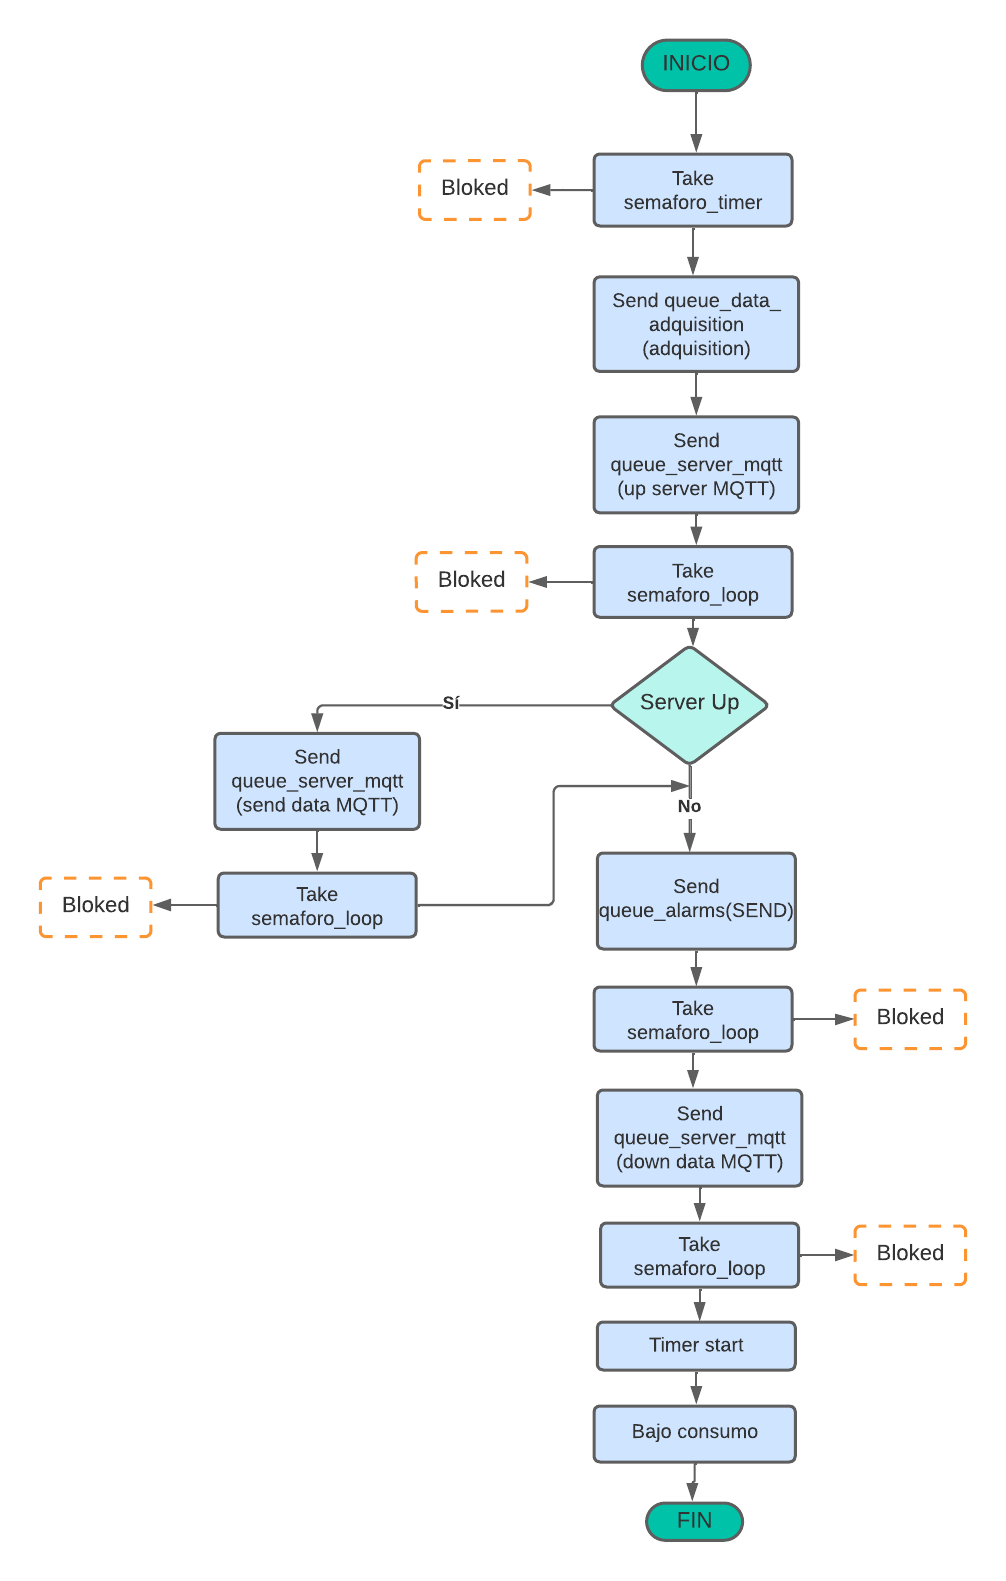
\includegraphics[width=1\textwidth]{./Figures/DF task loop.png}
	\caption{Diagrama de flujo tarea loop.}
	\label{fig:Df tarea loop sistema}
\end{figure}

La secuencialidad del sistema es manejado por la tarea de loop que nos permite tener secuencia repetitiva, la figura muestra el diagrma de flujo de la tarea loop 
La tarea comienza creando variables que se utilizaran localmente se inicia el timer del sistema, luego la tarea se blokea en el un semaforo esperando ser deblokeado por el un give que sera dado en el momento de la ejecucion del handler de la interrupcion del timer, luego se envia datos por las colas de adquisicion de datos y server mqtt para levantar el servidor y la tarea se vuelve a bloquear en el semaforos, cuando se desbloquea pregunta si se logro levantar el servidor si se logro se manda un mensaje por la cola de server mqtt con el evento de enviar datos y se bloquea nuevamente pero si no se logro levantar el servidor no se enviaran datos, luego se envia un evento a la cola de alarmas se bloquea nuevamente esperando que envien las alarmas, cuando se desbloquea el semaforo se manda un evento a la cola de server mqtt para desconectar el servidor y se bloquea la tarea en el semanforo esperando la desconexion  finalmente se inicia nuevamente el timer y mandamos al sistema a modo de bajo consumo. 


La figura muestra la secuencia repetiva que realiza la tarea de adquisicion de datos, la tarea inicia creando algunas variables locales que se utilizara en la tarea, luego entra al bucle infinito donde lo que promero que hace es ver si hay algun dato en la cola de adquisicion de datos si no hay se bloquea la tarea pero si hay realiza la lectura de todos los sensores, con los datos recolectados los envia a las colas de data y alarmas y termina el ciclo.
\begin{figure}[htbp]
  \centering
	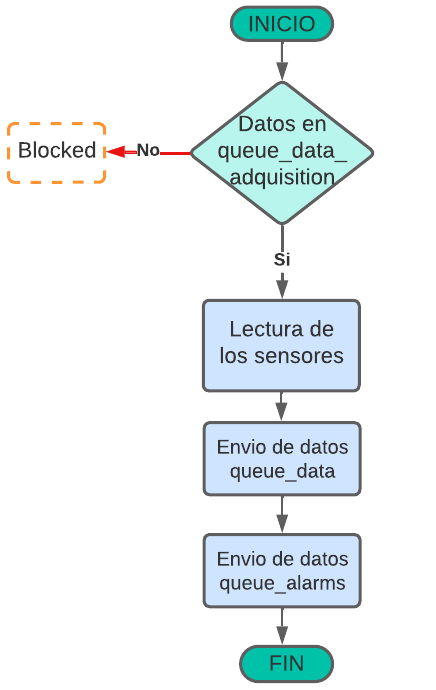
\includegraphics[width=10cm, height=8cm]{./Figures/DF task adquisicion.png}
	\caption{Diagrama de flujo tarea de adquisicion de datos.}
	\label{fig:Df tarea adquisicion}
\end{figure}

El manejo de las alarmas se realiza atraves de la tarea de alarmas la figura describe la secuencia de la tarea, 
al entrar al bucle infinito lo primero que se realiza es revisar si existe algun dato en la cola de alarmas si no hay datos la tarea se bloquea hasta que alguien envie un dato a la cola, si hay dato se pregunta que evento contiene el dato resivido por la cola si es de monitorear lo que se hace es ver si el dato del sensor de humedad es menor al rango esperado si es asi se una variable en alto advirtiendo al sistema que hay una alarma, si se recicivio el evento de enviar se revisa si hay alarmas activas si hay se envia un mensaje de texto al 

\begin{figure}[htbp]
  \centering
	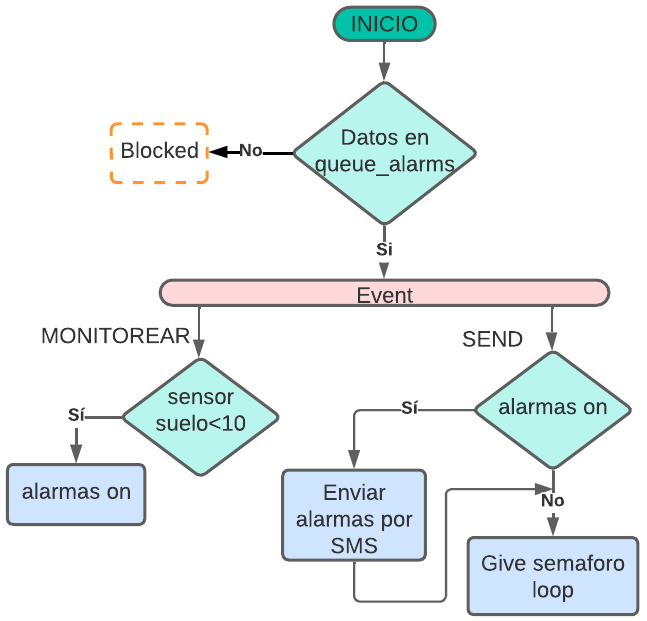
\includegraphics[width=8cm, height=8cm]{./Figures/DF_alarms.png}
	\caption{Diagrama de flujo tarea alarmas.}
	\label{fig:Df tarea alarms}
\end{figure}

La ultima tarea que implento es la tarea que maneja la conexion del servidor que se describe en la figura 
La tarea comienza esperando datos en la cola de servidor mqtt si no hay datos la tarea se bloquea, si hay datos se revisa que evento es el que se recibio tenemos tres posibles eventos UP, DOWN y SEND ,
si recivimos el evento de UP la tarea entra a una maquina de estados pra levantar el servidor la figura muestra la maquina de estados del evento UP, si el evento es de DOWN la tarea ejecuta la maquina de estados que se ve en la figura y el evento es SEND la tarea espera que existan datos en la cola de data para haci armar la trama y publicar los datos al borker MQTT.

\begin{figure}[htbp]
  \centering
	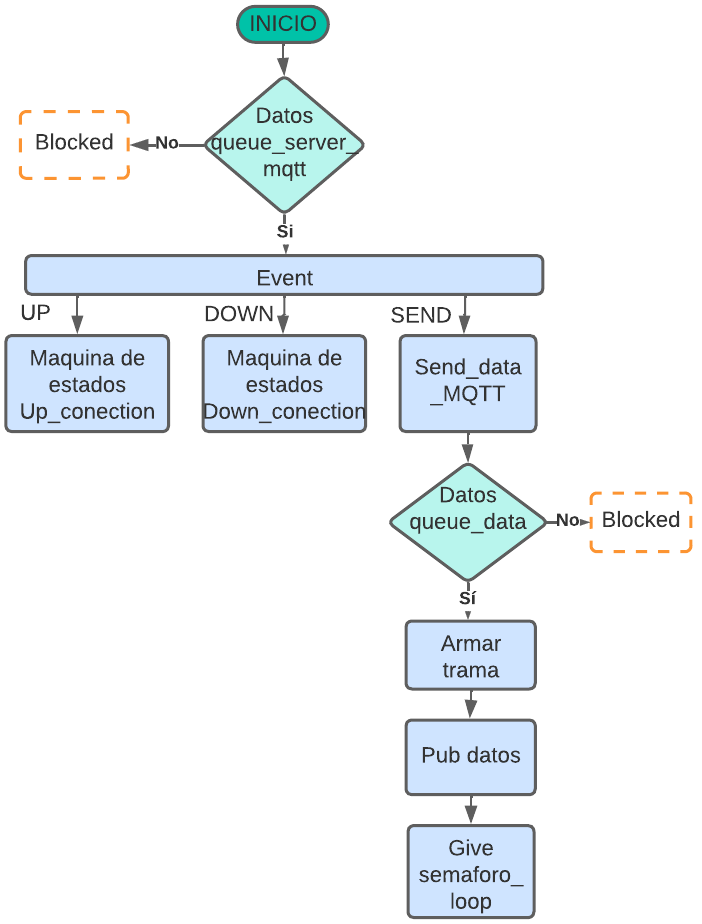
\includegraphics[width=8cm, height=8cm]{./Figures/DF general task conection.png}
	\caption{Diagrama de flujo tarea general conexion.}
	\label{fig:Df tarea conexion}
\end{figure}

\begin{figure}[htbp]
  \centering
	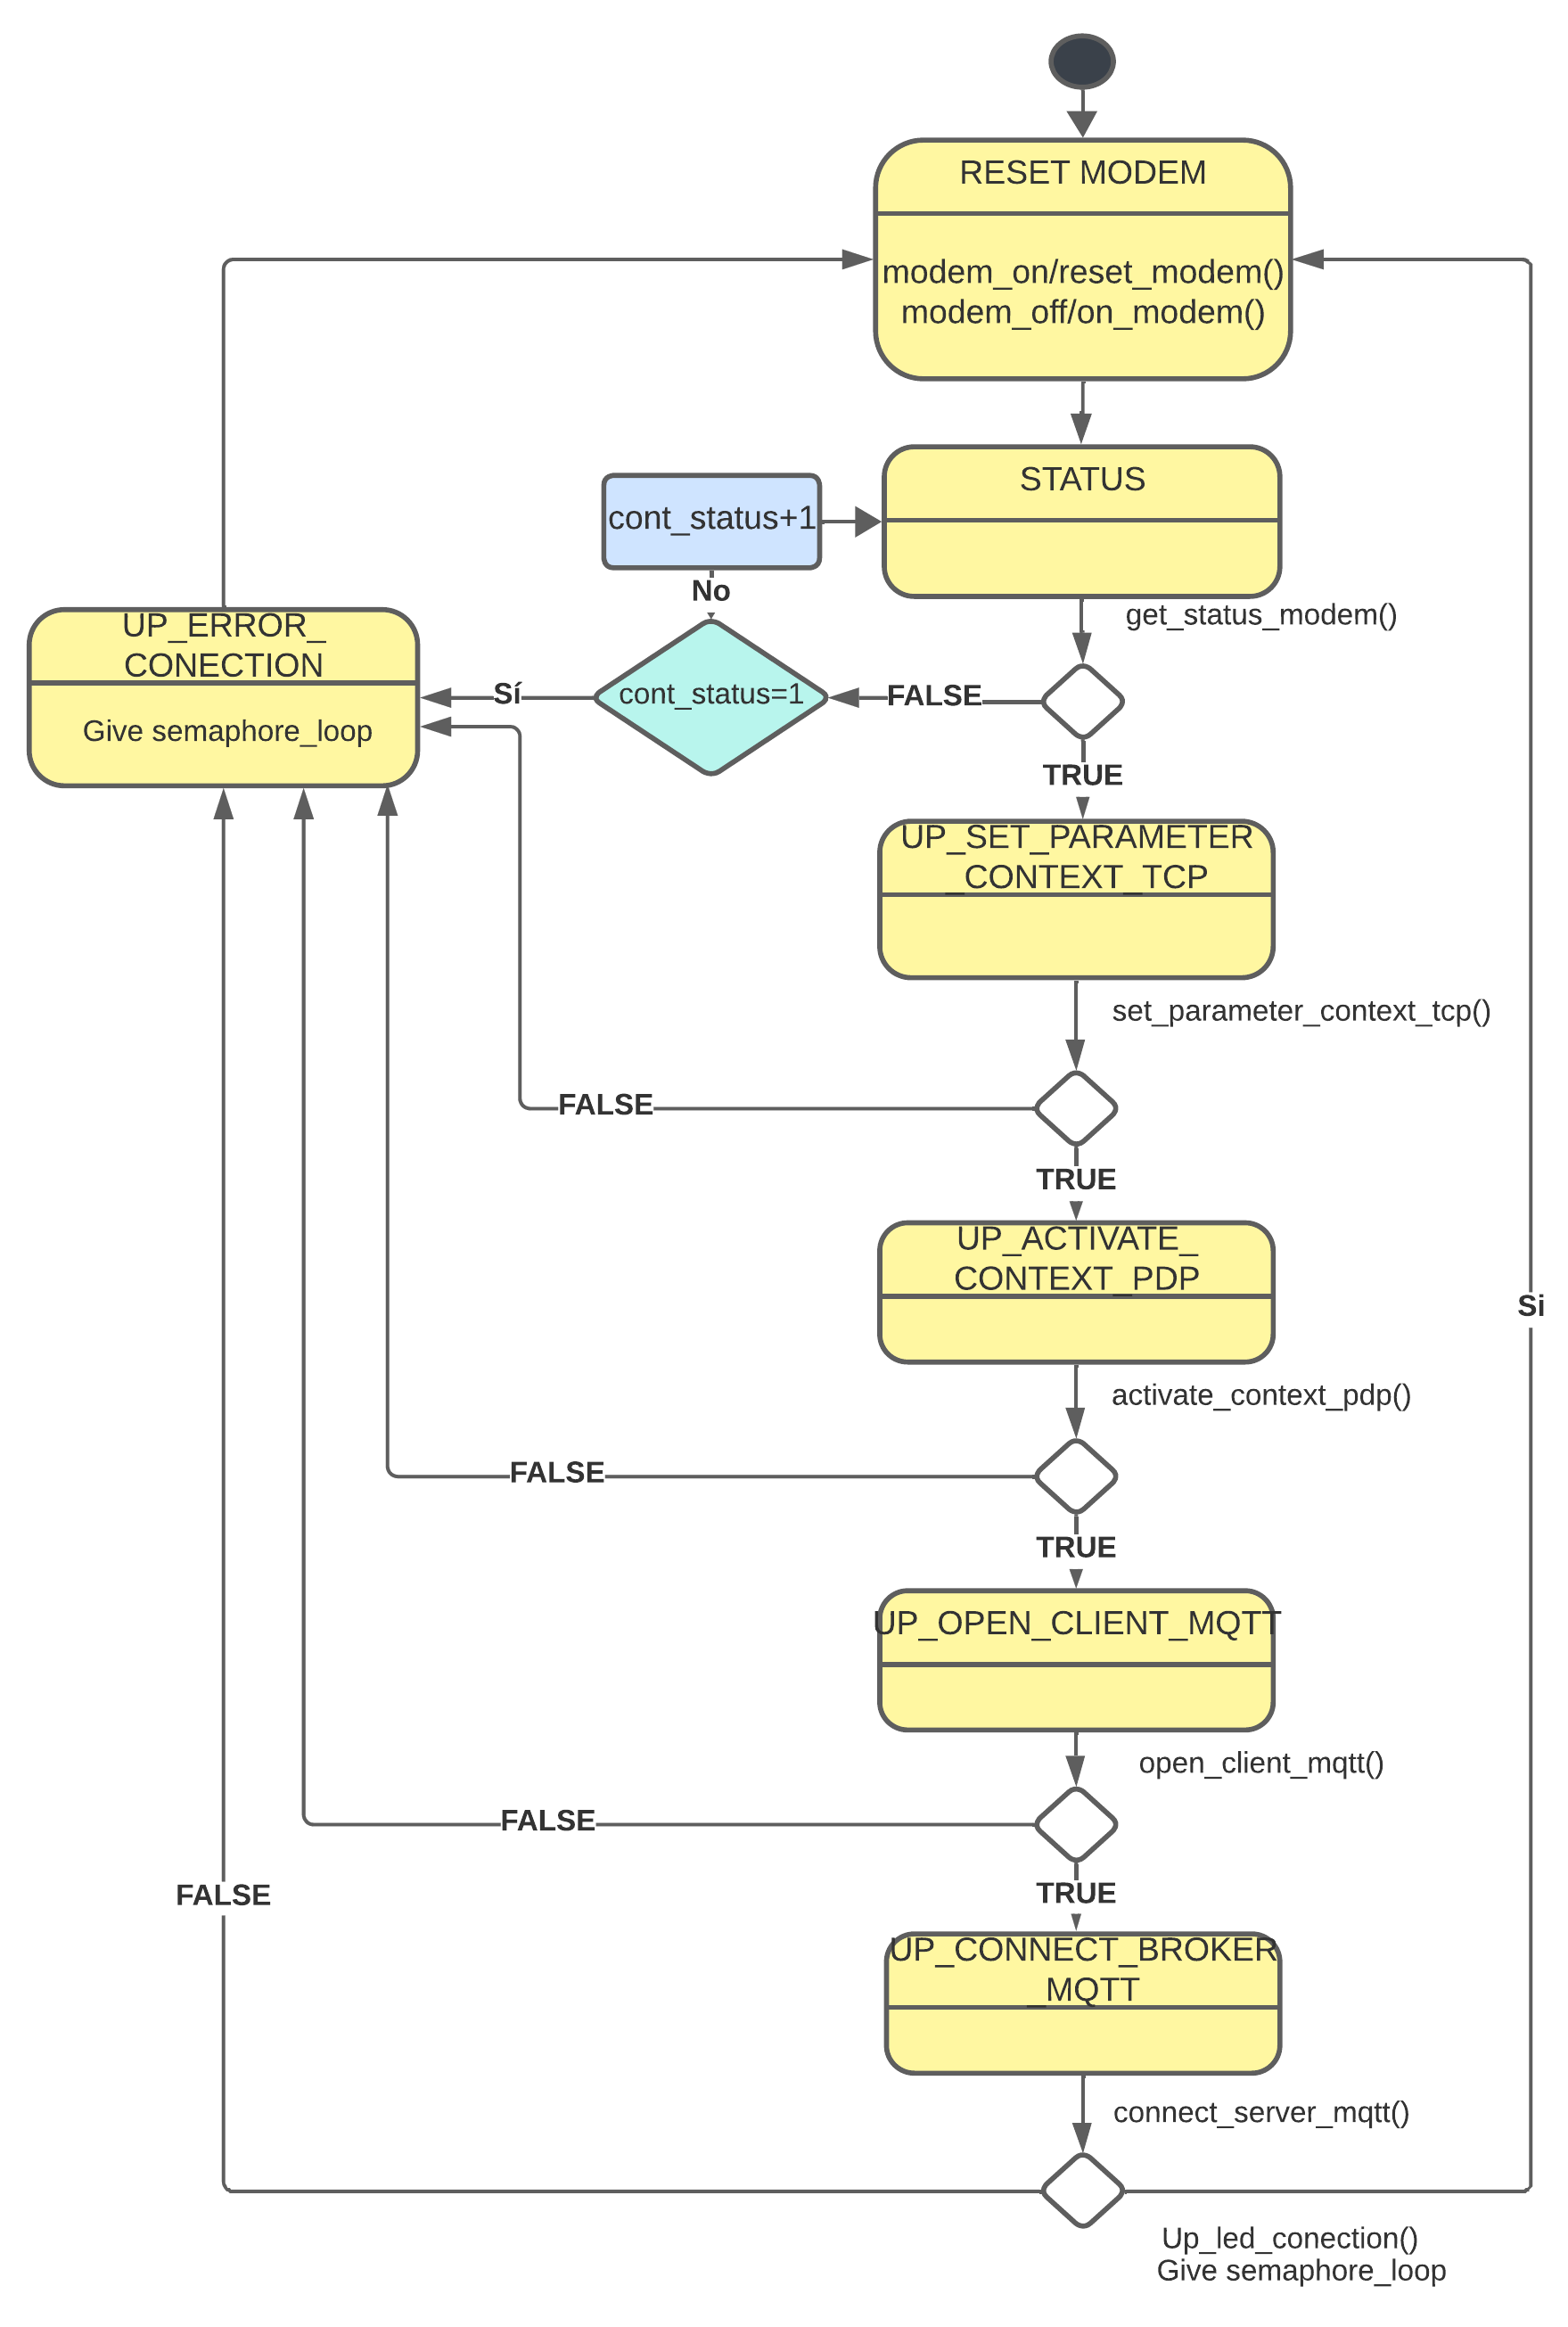
\includegraphics[width=10cm, height=15cm]{./Figures/SM up server.png}
	\caption{Maquina de estados up servidor.}
	\label{fig:Maquina de estados up servidor}
\end{figure}

\begin{figure}[htbp]
  \centering
	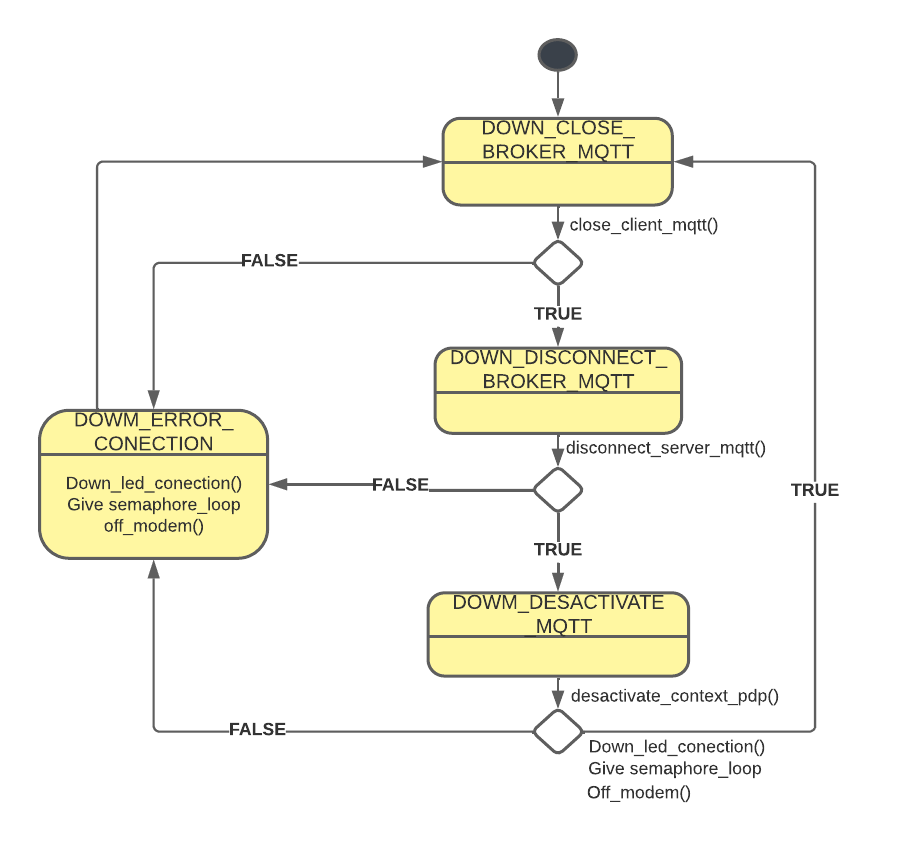
\includegraphics[width=8cm, height=8cm]{./Figures/SM down server.png}
	\caption{Maquina de estados dowm servidor.}
	\label{fig:Maquina de estados dowm servidor}
\end{figure}

\section{Desarrollo del hardware}

Lo que se hizo fue desarrollar un tarjeta donde se puedan conectar todos los modulos que se utilazaron para el prototipo
Al ser un prototipo no se realizon el diseno de un tarjeta con, lo que se hizo fue desarrollar un tarjeta donde se puedan conectar nuestros modulos utilizados como se el modulo celular, tarjeta de desarrollo STM32L432KC, los modulos sensores.

\begin{figure}[htbp]
  \centering
	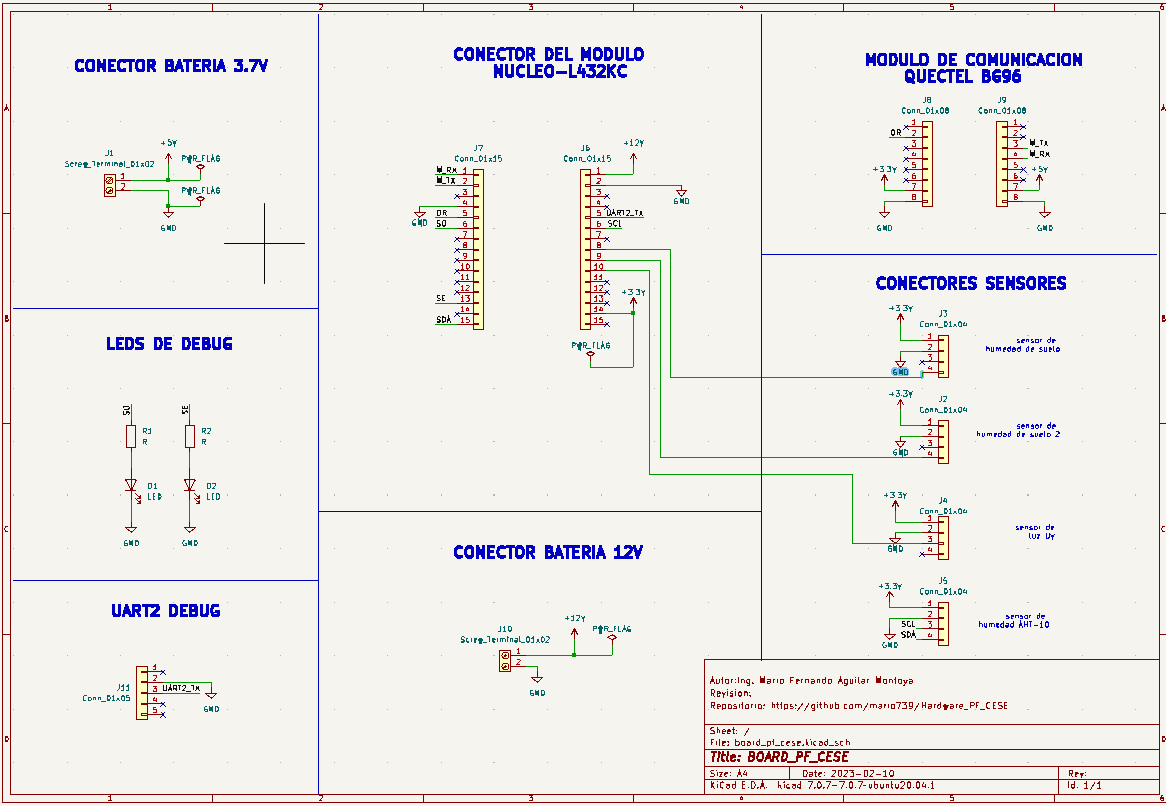
\includegraphics[width=20cm, height=\textwidth, angle=90]{./Figures/esquematico.png}
	\caption{Esquemaico del hardware.}
	\label{fig:esquematico}
\end{figure}

Descripcion de las partes del esquematico: 

\begin{itemize}
  \item Conector bateria 3.7v: Conector de la bateria 3.7v que alimenta el modulo de comunicacion bg96.
  \item Leds de debug: Se colocaron dos leds para debug, uno para senalizar si se logro conectar al servidor MQTT y el otro led para senalizar si el sistema entra en un estado de error.
  \item UART2 debug: Pines de conexion de conector uart, el firmware manda por este uart todos los comandos que manda al modulo de comunicacion y las repuestas del mismo.
  \item Conector modulo Nucleo-L432KC: Conectores para colocar el modulo a la tarjeta.
  \item Modulo de comunicacion BG96: Conector para colocar el modulo BG96.
  \item Conector de bateria 12v: Conector para la bateris de 12v que se utiliza para alimentar el modulo del microcontrolador.
  \item Conectores sensores: Son los conectores para los sensores utilizados.  
\end{itemize}

En la figura se muestra del diseno de la tarjeta del circuito impreso en 3D.
\begin{figure}[htbp]
  \centering
	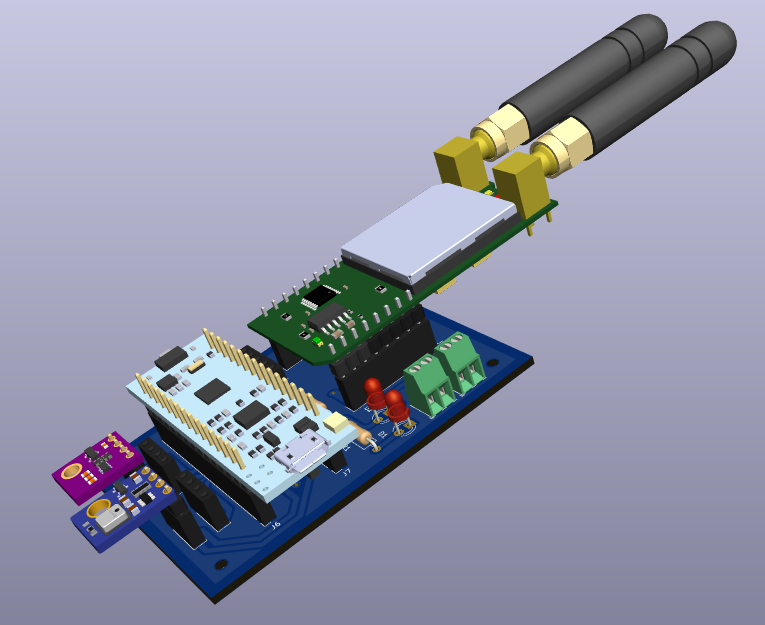
\includegraphics[width=\textwidth]{./Figures/tarjeta3d.png}
  \caption{3D del tarjeta desarrollada.}
	\label{fig:3D del modulo}
\end{figure}


\section{Interfaz de usuario}

Como plataforma IoT se utilizo ThingsBoard que nos permite hacer un desarrollo de una interfaz bastante completa y compleja, 

Para tener una interfaz escalable y bien distribuida se crearon dos panesles 

Panel principal 

En la figura se aprecia el panel principal.A la izquierda, en la parte superior un listado de todos los nodos sensores que estan implementados o se estan monitoreando asiendo click en el dispositivo podemos navegar a otro panel para visualizar los datos del nodo sensor.En la parte inferior izquierda tenemos una grafica que muestra algunas variables de los sensores,
y en l parte derecha del panel tenemos un mapa que muestra la ubicacion de los nodos sensores.


Para tener un mayor detalle de todos los parametros de moitoreo de cada sensor se creo un panel secundario que se muestra en la figura .
El panel secundario en la parte izquierda se tiene graficas de los valores que se van obteniendo de los sensores, en la aprte central tenemos el ultimo valor que se obtuvo de cada sensor, en la parte derecha superior del panel tenemos una tabla donde se muestran las alarmas que se activaron en el sistema y en la parte inferior derecha se tiene un mapa con la ubicacion donde se encuantra implementado el sensor.  
\begin{figure}[htbp]
  \centering
	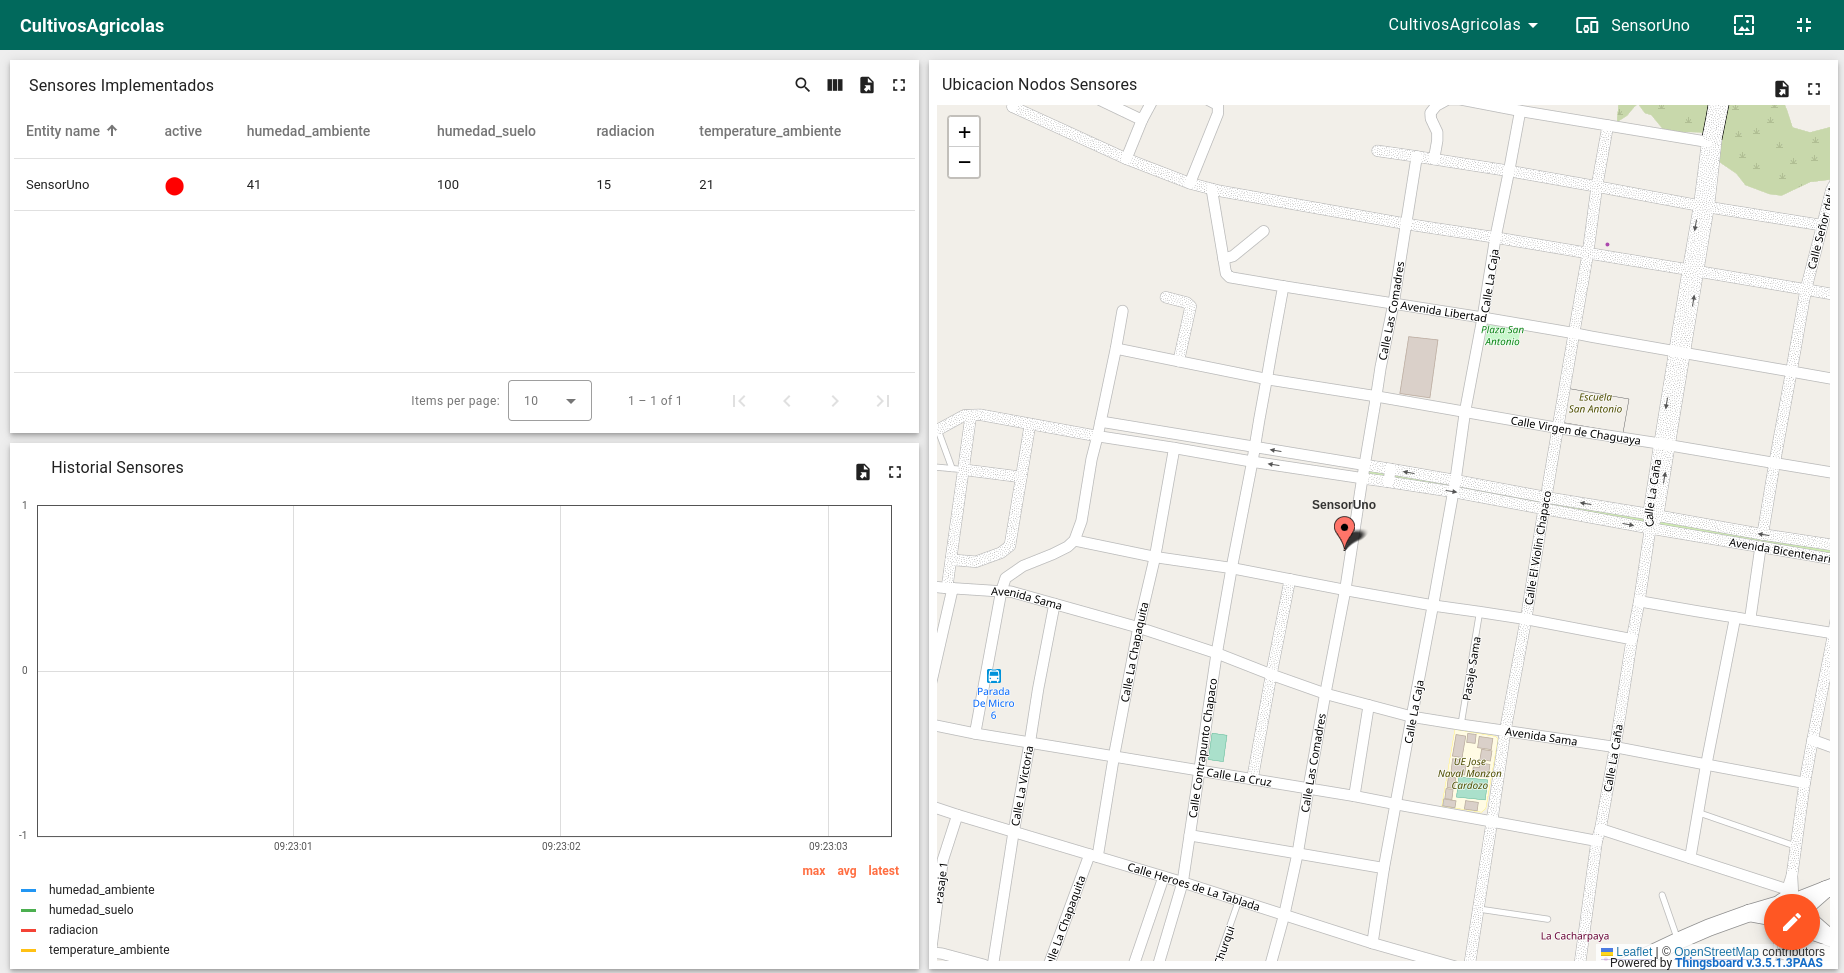
\includegraphics[width=\textwidth]{./Figures/panel_principal.png}
  \caption{Panel principal de la interfaz grafica.}
	\label{fig:Panel principal}
\end{figure}

\begin{figure}[htbp]
  \centering
	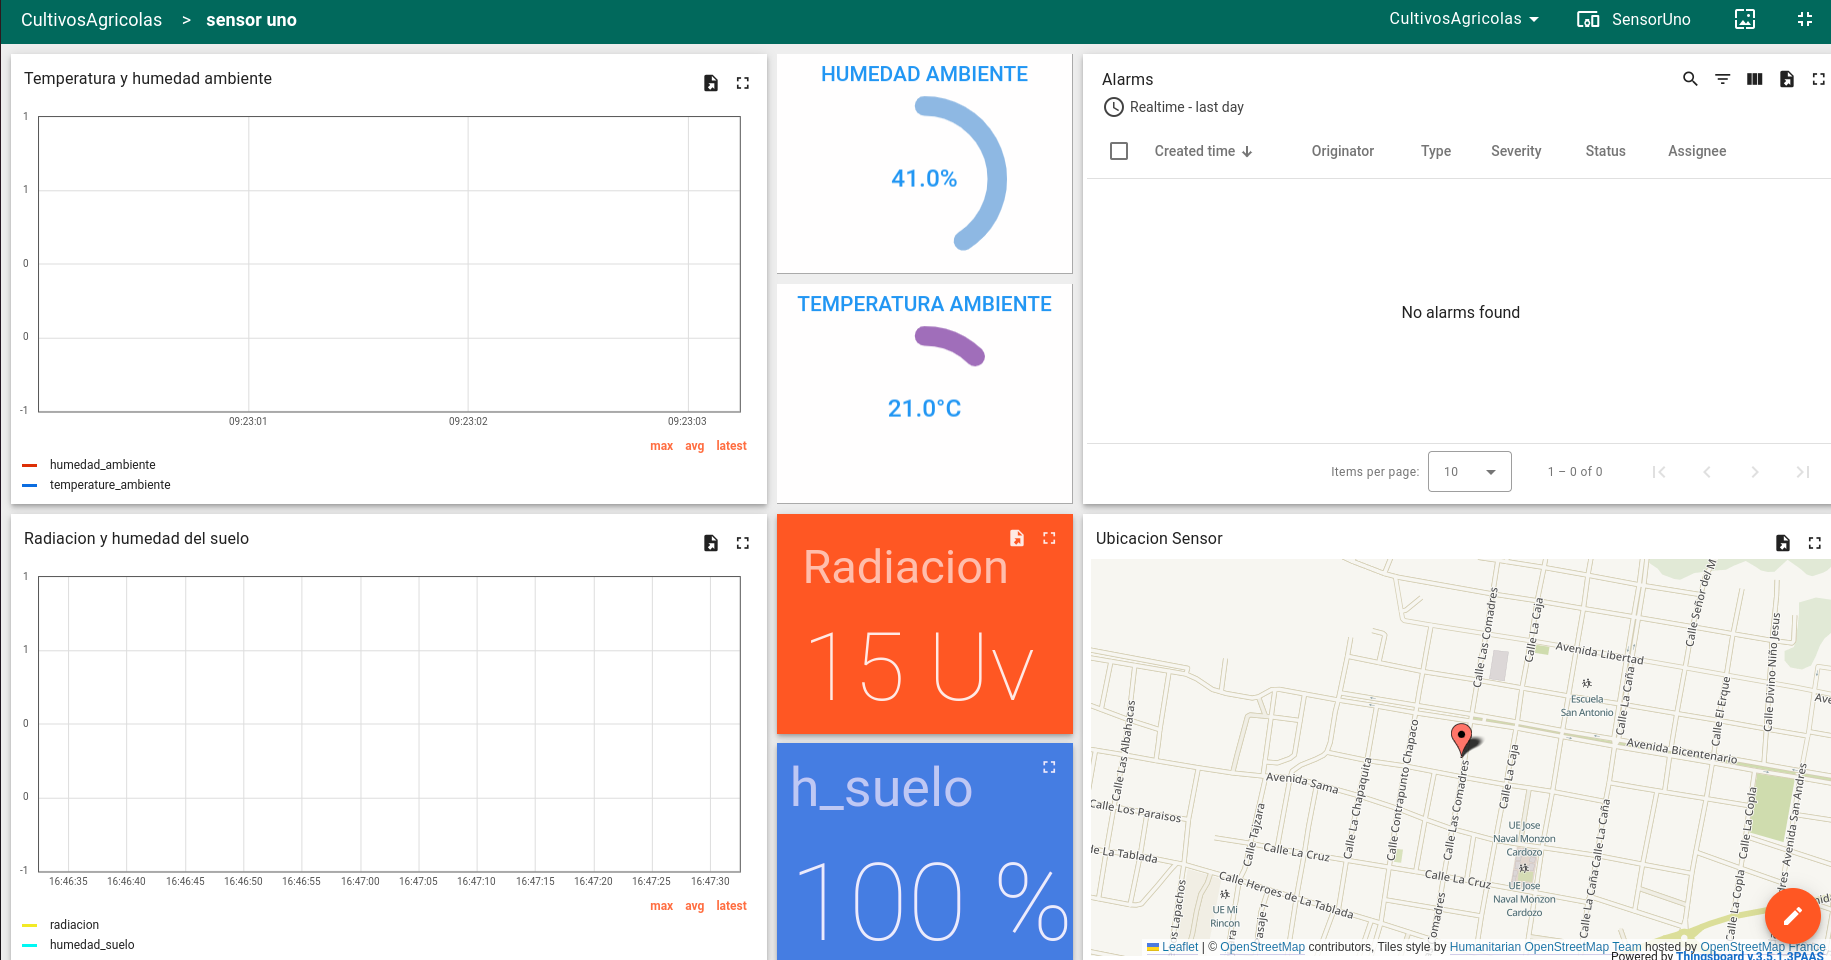
\includegraphics[width=\textwidth]{./Figures/panel_nodosensor.png}
  \caption{Panel nodo sensor.}
	\label{fig:Panel nodo sensor}
\end{figure}